\section{User Interface}
Considering the application is only a proof of concept (PoC) there is almost no focus on the user experience (UX) nor on the user interface (UI). To at least give a slight indication of what information needs to be displayed where, a UI mock-up is created in Adobe Xd, Adobe Xd is a lightweight, rudimentary visual editor that enables designers to quickly develop and share interactive prototypes. A few example screens of the UI prototype can be found below.
\begin{figure}[H]
\centering
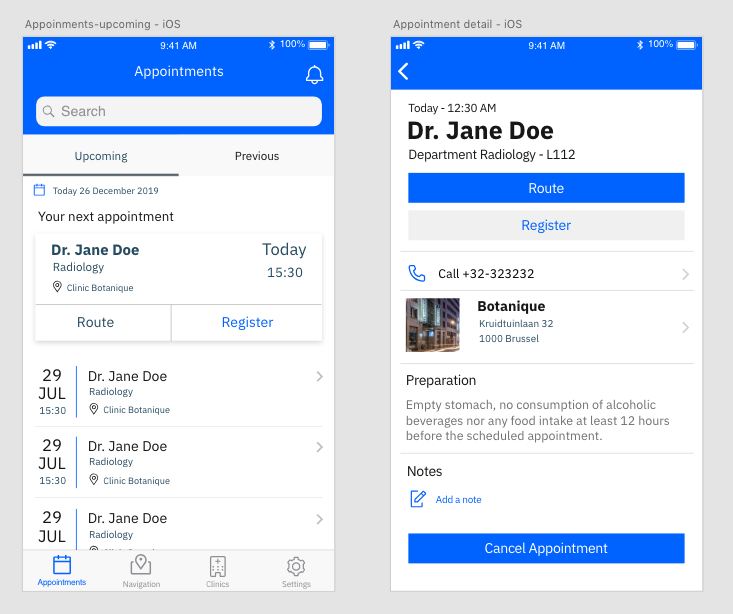
\includegraphics[scale=0.5]{appointments_screen_ios}
\caption{User interface of the appointments and detailed view for iOS}
\end{figure}
\begin{figure}[H]
\centering
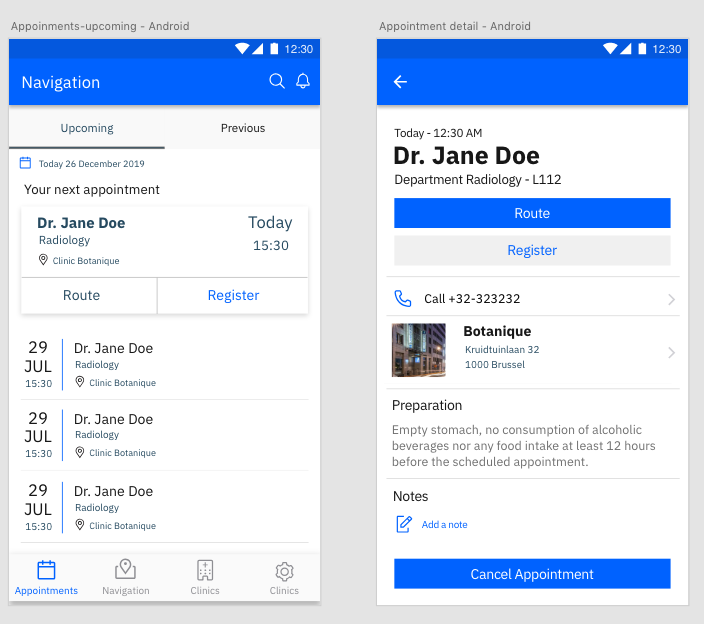
\includegraphics[scale=0.5]{appointments_screen_android}
\caption{User interface of the appointments and detailed view for Android}
\end{figure}
\begin{figure}[H]
\centering
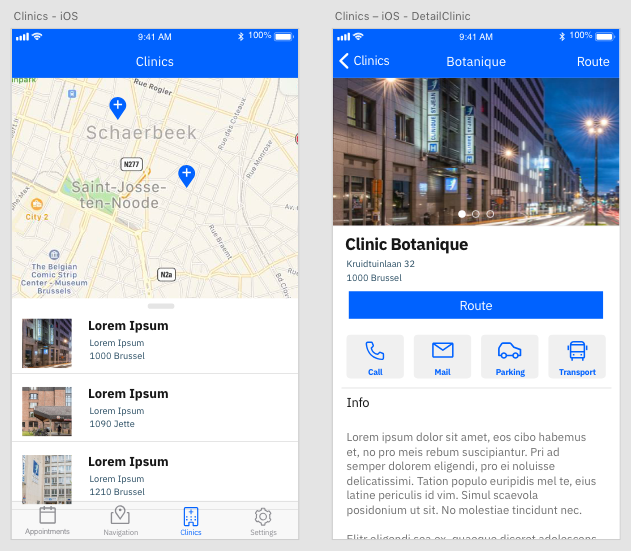
\includegraphics[scale=0.5]{clinics_screen_ios}
\caption{User interface of the hospital venues and detailed view for iOS}
\end{figure}
\begin{figure}[H]
\centering
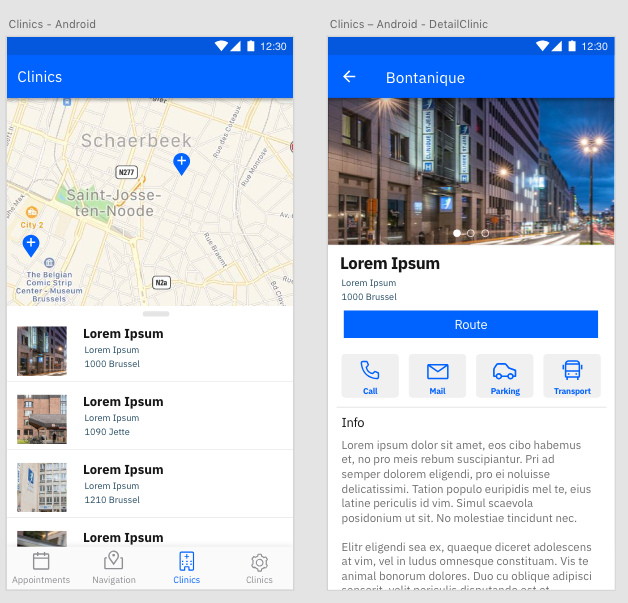
\includegraphics[scale=0.5]{clinics_screen_android}
\caption{User interface of the hospital venues and detailed view for Android}
\end{figure}
\section{Architecture}
The emphasis of the PoC is on developing it in such a way that it should be easy to re-implement the application elsewhere. The PoC is developed in the two current formats for mobile development: iOS and Android. This bachelor's thesis will cover the implementation of the Android architecture.
\subsection{General Architecture}
\subsubsection{Entities}
The specific entities used throughout this application are:
\begin{itemize}
\item appointment;
\item hospital;
\item venues - the different locations of a hospital;
\item address;
\item additionalinformation - meta for a hospital and venues;
\item department;
\end{itemize}
\subsubsection{UML Diagram}
\section{Database Communication}
\subsection{Testing API}
To aid in testing the database a test API is programmed using a Node.js framework: Express. it is a very simple tool to create web APIs ready for consumption \cite{Express2019}. The testing API is structured according to the entities specified in the UML diagram with the corresponding relations. For this specific application there a couple of endpoints exposed for requests:
\begin{itemize}
\item GET /appointments - this returns a JSON array containing test appointments;
\item GET /hospital - this returns information about the hospital such as address, contact details and venues;
\item GET /doctors - this fetches all the doctors present in the hospital records;
\item GET /departments - this returns all the departments available in the hospital and its venues;
\end{itemize}
\subsubsection{Faker}
Instead of using ad random numerical combinations or lorem ipsum texts, a library called Faker is used to generate different random values such are names, addresses, e-mail addresses and phone numbers. Faker is available for almost every general purpose language and is easy to use. It is always easier to work with representative data than it is to work with 'lorem ipsum' or '123456789' \cite{DanieleFaraglia2014}.
\section{Android Architecture}
\subsection{Separation of concern: Dependency Injection}
\subsection{Dependency Injection: Restaurant Analogy}
\subsection{Types of Dependency Injection}
\subsection{Type used in the mobile application}
\subsection{Dagger2 - Dependency Injection Library}
\subsection{Kotlin Language}
\subsection{Lifecycle Events}
For the duration of the runtime of the mobile application (from the moment the app is opened until it is closed) some events occur that are typical for an Android mobile application. A brief summary of these events is listed below (in chronological order) \cite{AndroidDeveloper2019}:
\begin{itemize}
\item onCreate() - When the activity is launched (This can happen after the onDestroy() event);
\item onStart() - When the activity is visible to the user;
\item onResume() - When the user returns to the activity after an onPause() event occurs;
\item onPause() - When activity is no longer visible;
\item onStop() - When the activity is finished or destroyed;
\item onRestart() - When the activity is restarted after a stoppage;
\item onDestroy() - When the activity is shut down;
\end{itemize}
\begin{figure}
\centering
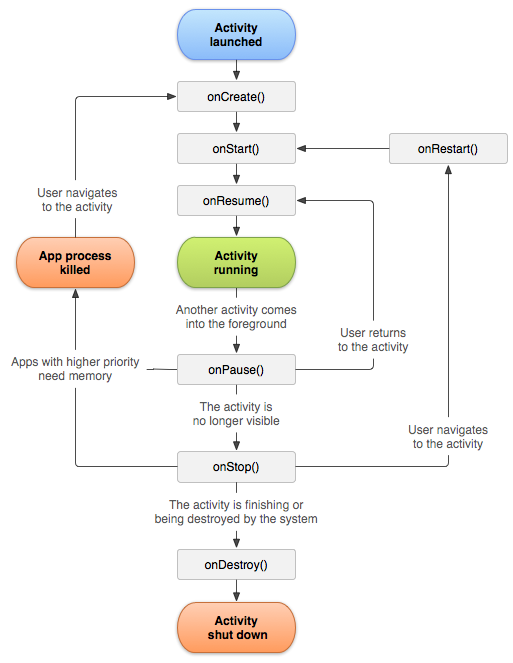
\includegraphics[scale=0.5]{activity_lifecycle}
\caption{Android Activity Lifecycle Schematic~\cite{AndroidDeveloper2019}}
\end{figure}
The lifecycle of an activity is an important factor to take into account whilst the application is being developed. This means a certain level of persistency is required for an optimal user experience.
\subsubsection{Bundles \& Saved State}
The way in which the onCreate() method is implemented allows a developer to declare a Bundle, which is an object that contains key-value pairs, that is used to restore an activity's previous state. If no such state exists then the Bundle will be equal to null. The Bundle object that is passed to an activity in the onCreate() method should only contain specific information such as user interactions: form fields, position on the screen and sometimes navigational properties. The main usage for this technology is when an activity gets paused or stopped, this means the OS (operating system) can freely destroy any activities \cite{JamesHalpern2012}.
\subsection{SQLite}
Another way to persist data throughout the lifecycle of an application is to use the (smart)phone's local storage. Each application can create a new local, file-based database using SQLite. SQLite is a transactional and serverless db (database), which means it is optimal for storing user-specific data. The fact that it is indeed a transactional db means that upon failing to save data it will rollback the entire operation \cite{TutorialsPoint2019}.
\section{Testing Application Programming Interface}
\section{Tools and frameworks used}
\section{MapWize}
MapWize is a service that digitalizes architectural plans and makes them interactive. The generated map from MapWize is the one used throughout the development of the application
for hospital CHC Saint-Jean in Liege. The main reason for using this service is to take care of the digital mapping of the hospital itself, which is not a task that should be completed by developers. The digital map will be used to show the routes from point A to point B, applied to this case: from the hospital's registration office to the place of appointment.
\subsection{MapWize SDK}
MapWize provides developers with a ready-made SDK for both iOS and Android. This SDK covers all important methods to 
\section{Cisco Connectected Mobile Experiences integration}
The manner in which the position of a patient is retrieved is based on the nearest WiFi router of Cisco.
\subsection{Function of Cisco CMX}
\section{IndoorLocation Framework}



